\section{VeloxDFS}
\subsection{Overview}

Contrary to what to a conventional description would be, I would prefer to
introduce \textbf{VeloxDFS} by deepen into \textbf{Apache Hadoop}.  As we have
discussed in the previous sections, one of the most important Big Data
processing framework is \textbf{Apache Hadoop} which At its very high level is
divided into two main logical components: The Hadoop File System and The
\textit{Hadoop MapReduce} (composed of other subsystems such as YARN, registry
and more essential services).  \\

\textbf{VeloxDFS} is the component of another framework named \textit{Velox Big
Data Framework} which similarly to \textbf{Apache Hadoop} has the same two main
levels: \textit{Velox MapReduce} or VMR, a MapReduce engine; and
\textbf{VeloxDFS}, a Distributed File System.  Nonetheless, \textbf{VeloxDFS}
can be also used with \textbf{Apache Hadoop} (substituting HDFS) by our
Velox-Hadoop API, and not only that, very interestingly, later versions of
\textbf{VeloxDFS} are solely compatible with Hadoop, there are many reasons
outside of the scope of this thesis for this decision\footnote{Sadly, a
\textbf{MapReduce} framework conveys a lot of work which due to our limitation
as a research lab we had to choose to narrow the scope of our requirements for
now. However, new students are starting to work in the \textbf{MapReduce}
level}  \\

As previously exposed a key difference with Hadoop file system is about the
elastic blocks, thus I would not deepen into this topic in this section. Other
key differences are regarding the topology of the network, while Hadoop uses a
standalone centralized network with a Namenode (and a quorum with High
Availability enabled), in  \textbf{VeloxDFS} each node is also a
\textit{namenode} for a small subsets of its files and blocks. We achieve this
by representing the nodes and the files in Distributed Hash table or
\textit{DHT} using CHORD-like protocol \cite{stoica2001chord} which ensures
safe node entering and joining while also statistically splitting each of the
file metadata evenly across the cluster. Also, similarly to HDFS we provide
data recovery by means of data redundancy using replicas stored in different
nodes.  \\ 

As for technical aspects the whole file systems is written in C++ for being
able to access Operating System low-level components and it network stack is
based on \textit{BOOST ASIO} using pro-actor model.

\subsection{Goals} 

As in many other parallel problems \textbf{MapReduce} systems can be quantified
by a set of variables which describes the system how well does the system
perform versus a different one.  In this work we focus in two key aspects: 

\begin{itemize} 

  \item \textbf{Job Execution time} that we try to tackle by
    reducing the variance of Task execution time in the Map phase.  

  \item \textbf{Load Balancing} that we try to tackle by shifting input data from
      straggling tasks to better performing tasks.  

\end{itemize}

It is important to mention that in many occasions, load balancing implies less
job execution time and vice versa. Thus, by attacking one of the goals we can
transitively achieve the second one.

\subsection{History}

Elastic blocks enabled \textbf{VeloxDFS} is the last iteration of many
iterations of the \textit{Velox Big Data framework}. The development of this
framework has taken several years and its genesis might be trace back to the
study of my  colleagues and I in a lesser manner regarding distributed
in-memory caches circa 2012 \cite{nam2012high} and later studies regarding
novel \textit{MapReduce} schedulers using \textit{\textbf{DHT}} caches
\cite{eom2015kde}. During those studies we have been considering the ideas to
of writing a MapReduce framework which benefits from all the lessons learning
during our studies of distributed cached and \textbf{MapReduce} cache aware
schedulers. For that purpose I participated in the implementation of a
prototype named EclipseMR \cite{sanchez2017eclipsemr} to deepen our studies and
to complete a prove of concept of our previous ideas into a real system.
EclipseMR was a major milestone in the project and implemented a
\textbf{MapReduce} engine which used an cache aware scheduler and a in-memory
\textbf{DHT} cache which its boundaries could be shifted to adjust to the
current system workload. This design proved exceptional, offering a greater
performance compared to other \textbf{MapReduce} systems such as Hadoop and
Spark in many of the single and multiple jobs standard benchmarks (such as
Terasort, WordCount, and Kmeans). EclipseMR was published at the IEEE Cluster
2017 at Honolulu, HW\cite{sanchez2017eclipsemr}\\

EclipseMR was a great piece of software that proved many of our ideas, however,
as in many successful software, EclipseMR was a victim of its own success. Its
fast development left a big technical debt which by the end of its first
internal release, adding non trivial features had become nearly impossible.
With this new situation, it became clear that we needed a new design and a new
project which was implemented in a more generic foundation in which we can
easily grow and iterate ideas. In 2015 we decided to go a step forward and
create an industry capable Big Data Framework utilizing all the novel
techniques used in our previous research and prototypes. The code-name for such
framework was Velox (From the Latin Fast). \\ 

Velox requirements were: Double-ring Distributed hash table shaped inmemory
cache and distributed filesystem; easily extensible design; Programmable client
API in Python, Java and C++; and most importantly iterative and DAG
\textbf{MapReduce} jobs support and iterative Maps work-flow. \\

Having all of those features in our backlog, I was assigned to design the
system as a whole and started the implementation in early 2015 with few more
colleagues. Concurrently, we enrolled an startup incubator program in where we
try to gain traction to our OSS Velox Big Data Framework and potentially find
ways to monetize our work similarly to many other Apache foundation Big Data
projects. \\ During that year most of our work was focus on finishing several
milestones to keep up with our funding budget and traction. \\

Unfortunately, while we implemented most of our backlog, due to multiple
technical issues the final performance was very poor compared to our rival
systems (Such as Hadoop and Spark). Our personnel to implement this system was
very limited, mostly composed of undergraduate and graduate students who can
participate in the code in their spare time. For all those reason, we gave up
the idea of finding monetary ways to our projects and moved towards narrowing
the scope of our requirements at the end of 2016. \\

We noticed that while the \textbf{MapReduce} engine was very
promising\footnote{We stalled the development of the \textbf{MapReduce} engine,
shortly after we finishing its first working version}, the Distributed file
system was easier to tweak due to its simplicity. In the summer of 2017
explored the idea of enhancing current \textbf{MapReduce} frameworks throughput
by using a custom underline Distributed file system which locates blocks at
more convenient positions. This idea has an strong inspiration from previous
works of some of my colleagues about reducing container initialization cost by
coalescing blocks in Hadoop\cite{kim2017coalescing}\\

For that purpose we moved an step forward and we decided to make
\textbf{VeloxDFS} to generate logical block distributions consisting on the
underline physical distributions. Those logical blocks can have arbitrary
sizes, customized by a new logical block scheduler engine embedded in each
FileLeader at the \textbf{VeloxDFS}. \\

After several iteration, we explored the idea about having arbitrary sized
logical blocks in which their size changes dynamically at run-time (While a
\textbf{MapReduce} job is running). Hence, for once we studied the idea of
elastic blocks distributed file system. This work explores in detail about this
idea and present what enhancement and challenges this idea brings.


\subsection{Architecture}

At its core, \textbf{VeloxDFS} is a decentralized \textit{userspace}
distributed file system written in C++.  A very important trait of this
FileSystem is that it relies in a Chord like protocol to index its files
metadata and its node information.  This is crutial as it provides a consistent
routing method to index its files and nodes while enabling nodes leaving and
entering the network witohut affecting its network consistency The file system
index its files on Chord-like Distributed Hash table, this is distributed
consistent hashing to index files and blocks across the different nodes and to
enable nodes leaving and entering the network with a safe manner\footnote{As
for November of 2018, the chord protocols for joining and exiting the network
are to be implemented and it our backlog. Reasons are that so far we are still
developing \textbf{VeloxDFS} and much of our efforts comes into finding novel
ways to distribute the blocks}.

\textbf{VeloxDFS} instances are designed based on the pro-actor pattern, as
result the server side reassembles an asynchronous RPC system. This was a key
decision early in the development which allows us to: avoid multithreading
while providing concurrency; use our in-house network library (libvelox) while
not locking \textbf{VeloxDFS} to it; and to separate business rules with
networking issues. \\

\subsubsection{File Metadata}

An essential component of any file system is how to deal with its file
metadata. To find effective ways to manage metadata we first need to understand
how it is and how it is used in \textbf{MapReduce} systems. In
\textbf{MapReduce} systems files are normally \textit{write once read many}
WORM, this give us a hint of how metadata is frequently accessed but rarely
written. Additionally, regarding its shape File Metadata is often much smaller
than the data its refer.\\ 

Consequently, both of the properties: being accessed frequently and being small
makes its a perfect candidate to be cached in memory and be easily indexed
using our Chord like \textbf{DHT} Filesystem. To deal with the peculiarities of
the metadata, we developed a complementary isolated component named FileLeader
which implements all the business logic regarding metadata store and
validation. It is very important to note that each file has its own FileLeader
which is determined by the position of its file name's hash value at the
\textbf{VeloxDFS} Distributed Hash Table range. \\

Fault recovery is done by FileLeaders gossiping its file metadata to its
nearest neighbors which in case of failure one of the would take over its Data
range and thus being able to reply any incoming query from clients. 

\subsubsection{Blocks and Chunks}

Recall from previous sections that we use the terms of Blocks to refer logical
blocks and chunks to refer to its underline small pieces of information that
compose those blocks. \\ One key aspect from those logical blocks is that they
change in size at any moment. To achieve that, their underline chunks would
loose the order, this is, the chunk 523 could be read after the chunk 5553.
This requires to split the chunks without spliting any of its records since if
we do not our tasks would incur in many remote reading calls which we try to
avoid at any cost. \\

A much better solution is to make the \texttt{upload} and \texttt{write}
function aware of the input file format so that it can split the input file
without spliting the blocks. We followed this approach and we only support line
record files at this very moment.

% TAlk about blocknodes

\subsubsection{Network}
Networking is the backbone of our distributed file system and it has some
peculiarities. Early on the design phase of this project much of the discussion
was focus regarding the problem of which technology stack to use for our
network parts. This was not an easy problem since using a very high level
technology such as a \textit{RPC} library while easing the development could
easily lock our system to a single technology and not let us perform fine
tuning, contrarily a very low level approach such as using \textit{TCP} or
\textit{UDP} sockets would make the development very long and error prone. \\

A middle solution was found with \textit{BOOST ASIO} and its proactor model,
this is by the fact that \textit{ASIO} is nothing else than a socket library
for \textit{TCP} with the support of a programming model named
\textit{proactor} \cite{pyarali1997proactor} pattern in which a Operating
system abstraction named \texttt{IO\_SERVICE} would hang a few threads and
released them to the specified functions by the user when an event (Such as a
incoming client action) is received. This library proved very suitable for our
purpose since ts  footprint is very small, its underline network low-level
primitives are accessible to the user, and more importantly pro-actor relies on
asynchronous operation which allows us to use a single thread per machine which
remove synchronization and race condition problems from our designs.

\subsubsection{API}

\textbf{VeloxDFS} can be interacted at two different levels, by using its C++
client library showed at the listing \ref{lst:API} and by using its
command-line utility command \texttt{veloxdfs} showed at the listing
\ref{lst:cli}. \\

\lstset{language=C++, basicstyle=\ttfamily\tiny, keywordstyle=\color{red},captionpos=b}
\begin{lstlisting}[caption=extracted from DFS.h, label={lst:API}, frame=tb]{name}
uint64_t write(std::string& file_name, const char* buf, uint64_t off, uint64_t len);
 
uint64_t read(std::string& file_name, char* buf, uint64_t off, uint64_t len);

int append(std::string file_name, std::string buf);

int upload(std::string file_name, bool is_binary);

bool exists(std::string);

bool touch(std::string);

int remove(std::string);

bool rename(std::string, std::string);

int format();

model::metadata get_metadata(std::string& fname);
\end{lstlisting}

\lstset{language=sh, basicstyle=\ttfamily\tiny, keywordstyle=\color{red},captionpos=b}
\begin{lstlisting}[caption=extracted from veloxdfs --help, label={lst:cli}, frame=tb]{name}
VELOXDFS (VELOX File System CLI client controler)
Usage: veloxdfs [options] <ACTIONS> FILE
ACTIONS
    put <FILE>               Upload a file
    get <FILE>               Download a file
    rm <FILE>                Remove a file
    cat <FILE>               Display a file's content
    show <FILE>              Show block location of a file
    ls -H|-g|-o [FILE]       List all the files
    format                   Format storage and metadata
    rename <FILE1> <FILE2>   Rename file 
    ...
Data Intensive Computing Lab at <SKKU/UNIST>, ROK. ver:1.8.6 Builded at: Oct 31 2018
\end{lstlisting}

\subsubsection{Logical block schedulers}

So far most of the conversation has skipped a very important idea, how and when
to change the logical block sizes. This is the task of the block scheduler
which upon its input and its logic will generate an optimal logical block
distribution based on its own heuristics of the system workload.

The remaining part of this work will focus on the following three block
schedulers and its evaluations. 

\begin{itemize}

    \item \textbf{Lean scheduler} which enables total or partial elastic blocks
      at run-time execution.

    \item \textbf{IO aware block scheduler} which generates a logical block
      distribution which mimics the monitored system load of the cluster.

    \item \textbf{Multiwave block scheduler} which generate multiple ever
      smaller waves of map tasks to address skewed tasks duration.

\end{itemize}

\subsection{Lean Scheduler}

The mechanism to assign the initial elastic blocks distribution and to control
its resizing is done by the \textit{lean scheduler}. The scheduler is situated
in both the client and the server side. In the server side the scheduler
arranges its initial block distributions explicitly at the Fileleader making
its best guesses using different techniques to construct logical blocks using
locally accessible physical blocks. The client side of the lean scheduler is
implemented at several levels: at the client side of \textbf{VeloxDFS} API to
Hadoop, at the \textbf{VeloxDFS} client API, and at a Distributed lock system
instance. 

Due to the fact of having two types of schedules call, one initial and one (or
more) at run-time, we need a way to partition the input data among the
different scheduler calls. At the highest level, We split the input data into
two segments: one for the initial block assignment and the remaining input data
for the consequently run-time elastic block adjustment. The initial block
assignment percentage is noted as $\alpha$ in this description

\subsubsection{Server side lean scheduler}

The server side of the lean scheduler competence is to write the initial
physical blocks to logical blocks mappings, e.g. the initial logical block
distributions. This scheduler invocation is done at the target file's
\texttt{FileLeader}. As explained in the previous section the server side of
the lean scheduler will commit a certain percentage $\alpha$ such that: $\alpha
= \{0.00..1.00\}$ of the input data during the initial phase. In this phase
given $N$ chunks for our input file, this server side scheduler will assign
$\alpha N$ chunks of the file in round robin manner to the servers containing
each replicas. 

\subsubsection{Client side lean scheduler}

The client side of the lean scheduler competence is to dynamically adjust the
initially given logical blocks. This adjustment takes places after $\alphaN$
has been processed. To understand how this client side run-time adjustment
works. Every tasks continuously request more data to read, in our client DFS
layer when we finished reading the presassing chunk, the client knows every
chunks that its located locally. With that information before trying to process
it, it will create a lock in the distributed lock system so that other tasks
containing the replica will abstain from processing the chunk generating
redundant computantions such as in the case of Hadoop with speculative maps.
There are several implication of using a distributed lock system, the very
important one is regarding overhead, through this paper we deepen into this
idea and we offer some solutions in the form of tuning and future ideas.

%The run-time block adjustments is done by dynamically assigning physical
%blocks to the current logical blocks. This is, whenever a tasks finishes with
%a physical block it will then attempt to process another physical block's
%replica. Since there are multiple replicas we can consider that the slot with
%the highest throughput is more likely to process one of the physical blocks's
%replicas. Also, having this redundancy creates the need to have some sort of
%synchronization technique in the form of lock. In our work, we use a
%distributed lock system with as much locks as physical blocks, in the
%following section we will cover the overhead consideration of this design.



\subsubsection{Overhead considerations}

The design of the lean scheduler obviates a particular bottleneck located at
the distributed lock system. Such distributed lock system must maintain as much
locks as physical chunks in the file that we are currently processing.
Additionally, each of the tasks would concurrently attempt to lock the locks of
its assigned physical chunks. This can be a problem when we scale our cluster
to have more then 10000 slots, with each slots having hundreds of physical
chunks. Several approaches can be determined such as partitioning the locks
across multiple nodes, and buffering the lock request a transaction of multiple
requests.  

\subsection{Job-static schedulers}

Our earlier approaches where based on the idea that we can only generate an
static block distribution which can not be changed while the job is running.
The reason was solely based on the implementation issues, our initial Hadoop
API consisted in a FileSystem API so that Hadoop would internally call Velox
during the job in the same manner as it interacts with HDFS. The main drawback
with this approach is that by default jobs in Hadoop only ask once at the
beginning regarding the block locations and its sizes. This seriously limited
our degree of action and restricted our logical scheduler to only have one
chance of generating a logical block distribution. \\

Having in mind this strong limitation, we first explored the idea of monitoring
the system workload in each of the servers and generate a block distribution
countering this system workload to later explore the idea of generating logical
block distributions base on an interesting find of how tasks ending time
differs on average.

\subsubsection{IO aware block scheduler}

The first block scheduler that we considered created logical block
distributions upon of the current IO/CPU workload of the given cluster. For
that purpose, we collected Exponential Weighted Moving Averages (EWMA) of the
current IO usage percentage obtained from UNIX tools such as \texttt{iostat}
for every machine in a cluster every certain time paramitrezable for the user.
We also kept track of the load average of each machine to determine how many
free cores each server has on average in the past few minutes, this
architecture can be visualize at the figure\ref{fig:ioaware_arch}.  Upon given
this information to the IO aware schedule, the IO aware scheduler will generate
a logical block distribution which mimics the cluster-wide system load. \\ 

The exact way of how this block distribution was generated can be seen at the
listing \ref{fig:ioaware_alg} in which given the few servers containing each of
the replicas of a chunk. Only the server with the high score will get the
replica assigned. This score considered local system IO. local system workload,
and very importantly a ration of current assingned chunk v.s other servers.

\lstset{language=C++, basicstyle=\ttfamily\tiny, keywordstyle=\color{red},captionpos=b}
\begin{figure}[htbp]
\begin{tabular}{p{0.5\textwidth}p{0.5\textwidth}}
    \begin{minipage}{.5\textwidth}
    \centering
    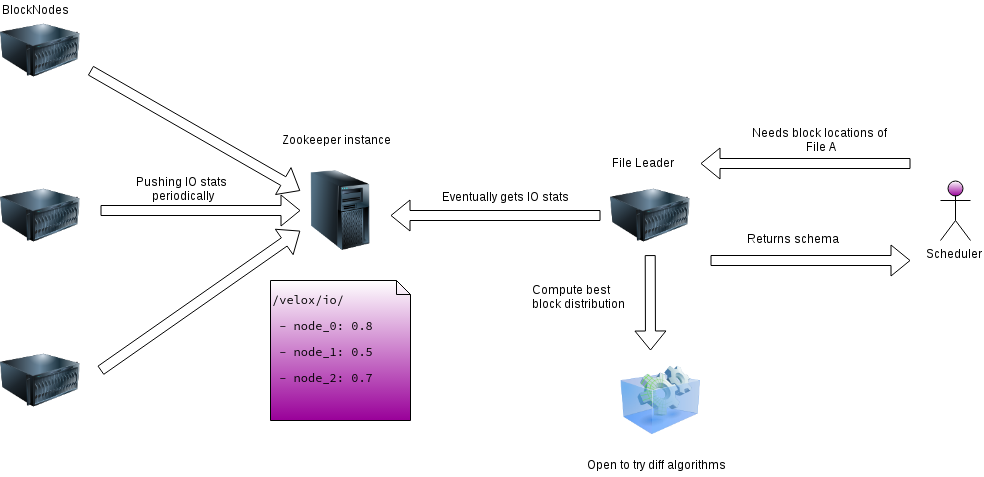
\includegraphics[width=1.0\textwidth]{figures/ioaware_architecture.png}
    \caption{IO monitoring architecture}
    \label{fig:ioaware_arch}
    \end{minipage}
    &
    \begin{minipage}{.5\textwidth}
    \begin{lstlisting}
double score(int id) {
  double alpha = get_alpha();
  double beta = get_beta();
  double delta = 1.00 - alpha - beta;
  double io = get_io();
  double load = get_sysload();

  return 1.00 - (delta*usage[id] + 
                 io[id]*alpha +
                 load[id]*beta);
}

int get_highest_id(VEC_INT nodes_containing_replicas) {
  vector<double> score_vec;

  // We get each replicas' score
  for (auto node_id : node_containing_replicas) {
    score_vec = score(node_id);
  }
 
  // Finally get the id of the highest replica's score
  return max_element(score_vec.begin(), score_vec.end());
}
\end{lstlisting}
\caption{IO aware score algorithm}
\label{fig:ioaware_alg}
\end{minipage}
\end{tabular}
\end{figure}


\subsubsection{Multiwave block scheduler}

A breakthrough came into the form of realizing that most of our observed
\textbf{MapReduce} Job's tasks ending time had an around 20\% variance --also
seen at the last figure at the grid \ref{fig:lean_grid}. This inspired the
creation of the multiwave block scheduler which addresses this problem by
creating ever smaller logical blocks to produce ever smaller map waves which in
theory would reduce this tail problem at the tasks ending time previously
mentioned. \\

The idea is that it takes only a straggling task to delay the whole job
execution time. The approach to fix this was to generate a logical block
distribution consisting in initial large logical blocks followed by one or more
waves of recursively smaller logical blocks. By doing that we hoped Hadoop to
start scheduling those large blocks first and start allocating the smaller
blocks in the slots which are free (this is, the good performing slots). \\

This idea gave good load balance results, however, often Hadoop would not honor
our request to schedule first the large logical blocks sabotaging our idea and
finally rendering our idea useless.

\lstset{language=C++, basicstyle=\ttfamily\tiny, keywordstyle=\color{red},captionpos=b, linewidth=0.5\textwidth}
\begin{wrapfigure}{r}{0.5\textwidth}
\begin{lstlisting}[caption=Recursivily generate waves, label={lst:recursive}, frame=tb]{name}
const int MIN_BLOCK_SIZE = 8 // MiB
const int CHUNK_SIZE = 4     // MiB

bool schedule(int SLOTS[], int CHUNKS[]) {
  if (LEN(CHUNKS)/LEN(SLOTS) * CHUNK_SIZE < MIN_BLOCK_SIZE) {
      return false;
  }

  int *C_1, *C_2;

  split_chunks(CHUNKS, &C_1, &C_2);

  if (!schedule(SLOTS, C_2)) {
     arr_append(&C_1, C_2);
  }

  assign_chunks_to_slots(SLOTS, C_1);

  return true;
}
\end{lstlisting}
\end{wrapfigure}

\subsection{Additional components}

As previously mentioned, \textbf{VeloxDFS} should not be seen as a single
monolithic piece of software, rather, as a composite of many small component
working together. This architecture follows the UNIX philosophy of decomposing
your program into small programs which perform a single operation very well to
gain the flexibility of later being able to expand your system without
signficantly increasing its complexity. \\ 

Since this work is focus on the research per se and not the underline software
I would briefly describe the main component of \textbf{VeloxDFS} in the
following table with links to its Repository pages 

\begin{table}
\footnotesize{}
\centering
\begin{tabular}{ |c|c|c| } 
 \hline
Project                               & Description                  & GitHub URL  \\
 \hline
VeloxMR           &  Experimental MapReduce engine based on VeloxDFS & DICL/VeloxMR \\
 \hline
eclipsed          & Deployment/debugging helper script & DICL/eclipsed \\
 \hline
velox-hadoop      & VeloxDFS JAVA library for Hadoop                 & DICL/velox-hadoop \\
 \hline
velox-deploy-ansible & Automatize deployment of VeloxDFS & DICL/velox-deploy-ansible \\
 \hline
hadoop-etc        & Hadoop configuration files to use VeloxDFS       & vicentebolea/hadoop-etc \\
 \hline
velox-report      & Suit to Benchmark, profile and log VeloxDFS & vicentebolea/velox-report \\
 \hline
\end{tabular}
\label{tab:ecosystem}
\end{table}
